
\chapter{The "XYZ" Prototype System}
%\index{TODO CHANGE: XYZ}
% NOTES / TODOs:
%
% Architecture scheme, implementation
% callback functions, hot plugin
% js-select selectors
% List of condition operators
% Why JS, why wasnt it used before? is it used now?
% Terminierungsproblem (compiler bau), loesungsansaetze

% Required use cases since their application was promised before in the thesis:
% smart filtering
% aggregation of information in whatever location user wants
% 

% as seen by user,
% as seen by developer

The "XYZ" prototype system is the realisation of a reactive web system.
It was developped during the research for this thesis and acts as a platform for feasibility studies of certain use cases.




\section{Architecture}
"XYZ" consists of a queue in which all incoming events are pushed, and an engine that picks the events from the end of the queue whenever it is idle.
Since "XYZ"'s core functionalty is the communication with resources in the web, the architecture bases on HTTP protocol in several parts.
For example the events are meant to be retrieved completely via HTTP, the user interface is a webpage which posts requests to the system and most actions are also meant to be HTTP requests, or at least using them to gather information.

\begin{figure}[!ht]
	\centering
  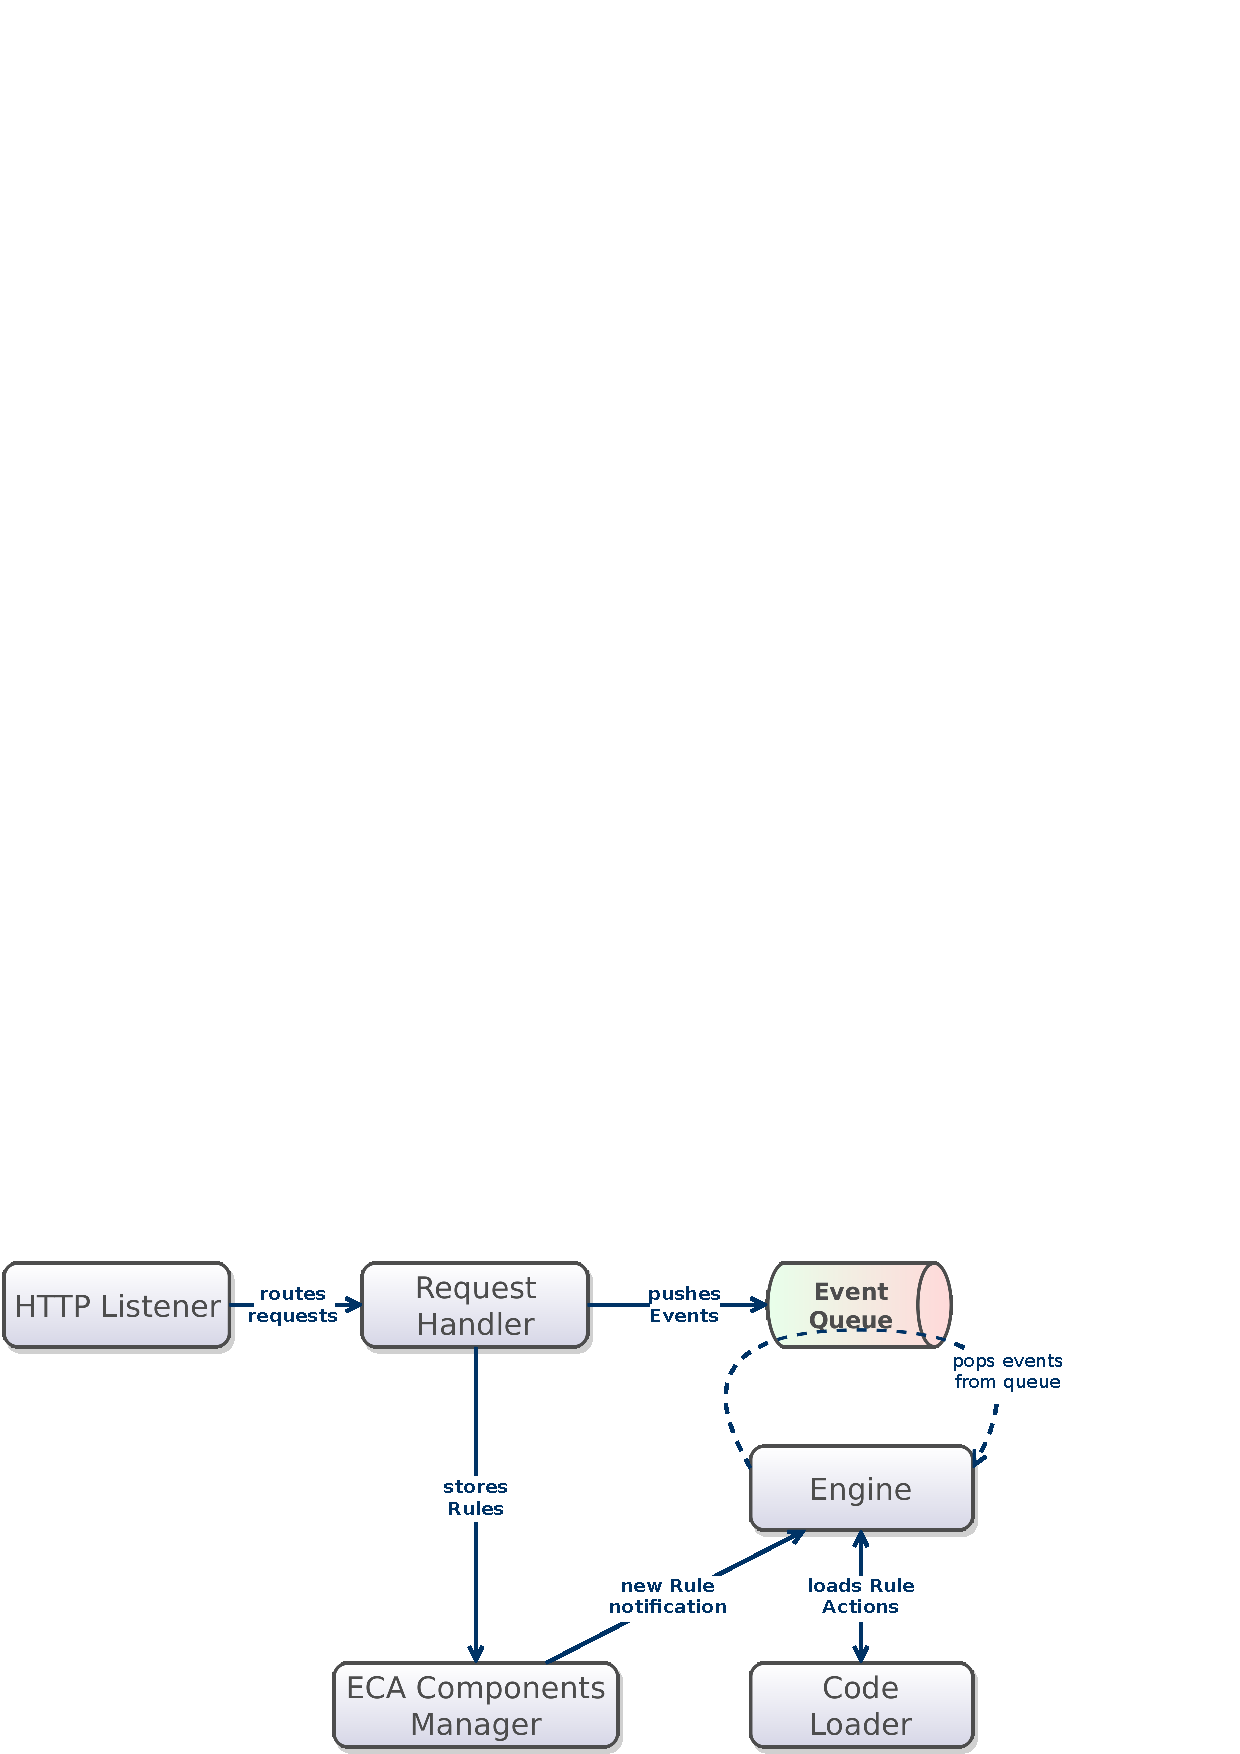
\includegraphics[width=0.8\textwidth]{figures/Architecture_woET}
	\caption{"XYZ" Architecture}
	\label{fig:Architecture_woEP}
\end{figure}

\begin{figure}[!ht]
	\centering
  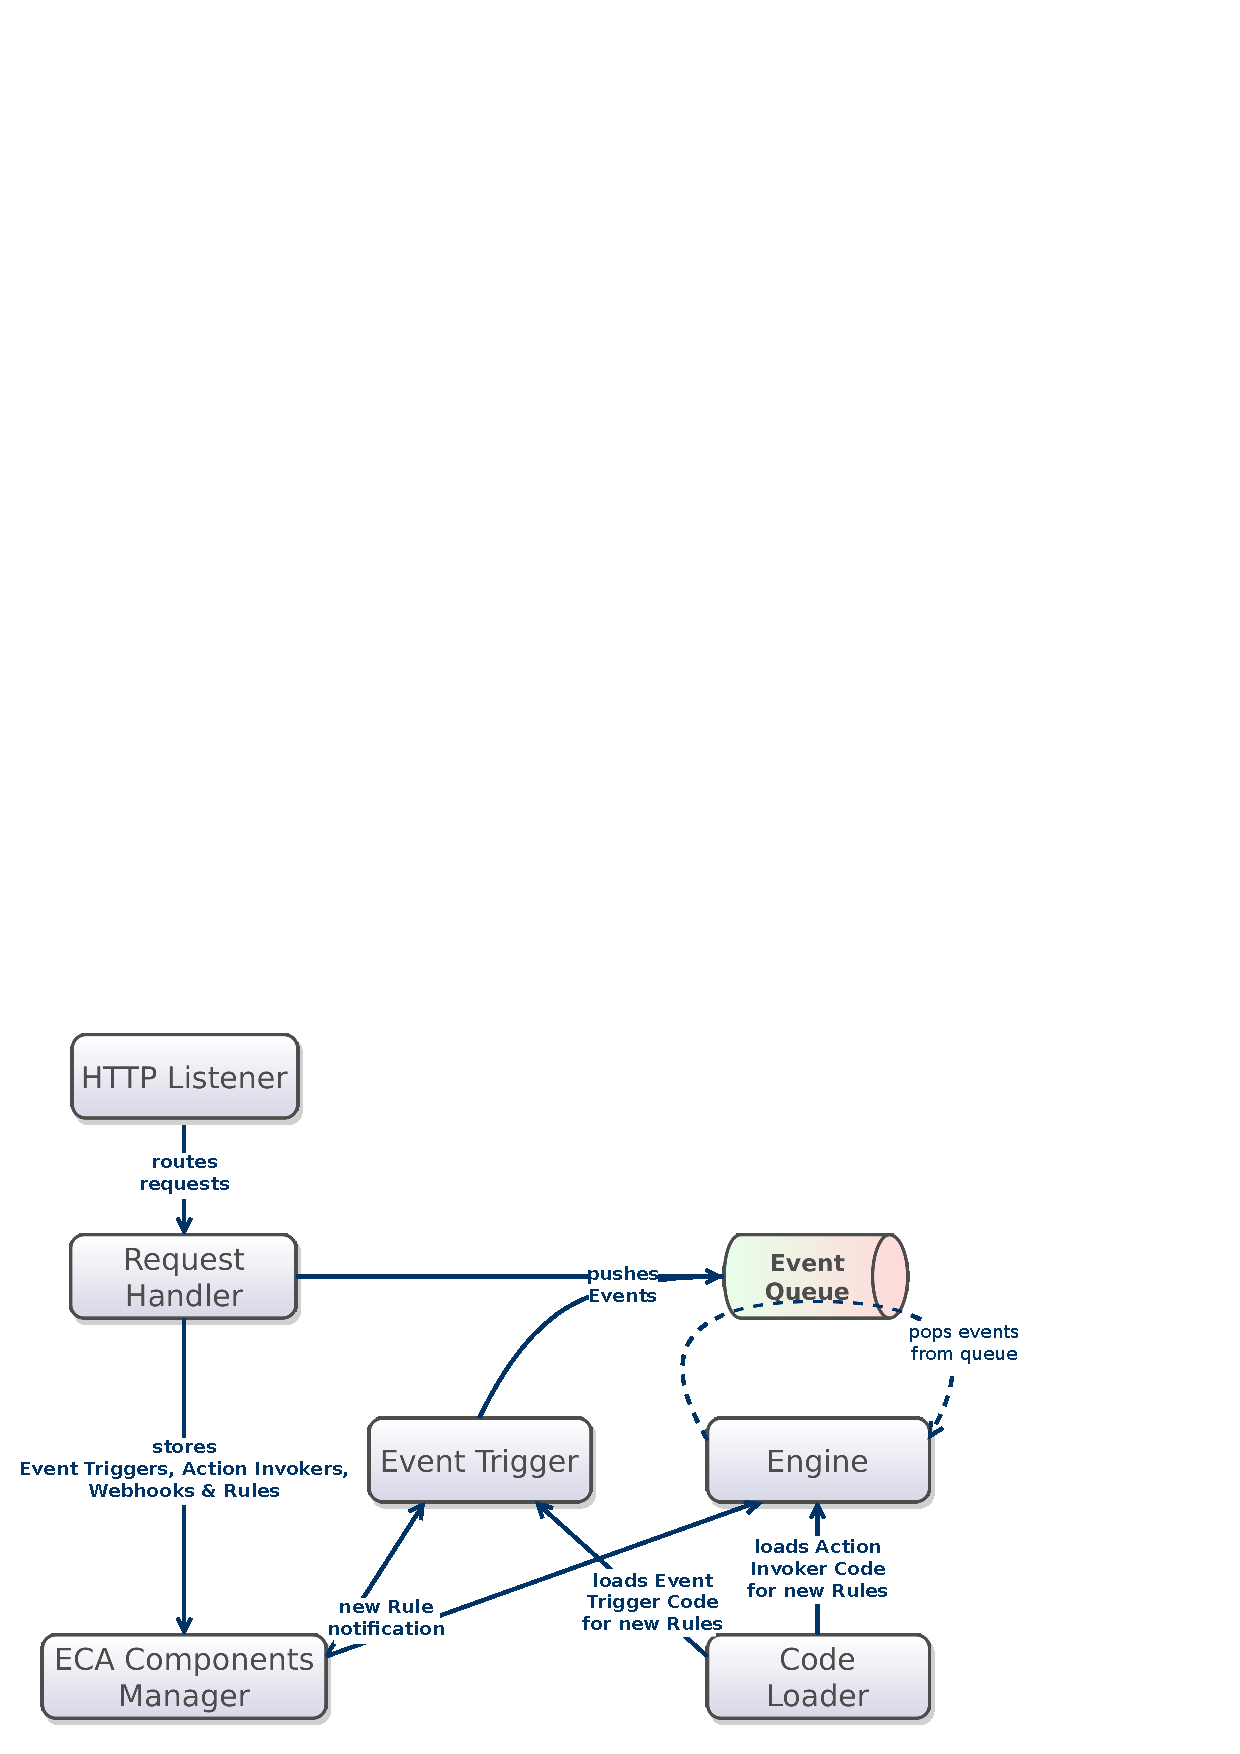
\includegraphics[width=0.9\textwidth]{figures/Architecture_wET}
	\caption{"XYZ" Architecture}
	\label{fig:Architecture_wET}
\end{figure}


\section{Event Trigger}

Event Gathering is the E in ECA and without one of these letters such a system would not run.
It is of utmost importance to find as much as possible ways to get data into a system.



\subsection{Polling}

\subsection{Webhooks}







\section{Action Invoker}

% Not only from events
% import.io

\section{ECA Rules in the Engine}
% TODO Conditions
% Explain rules, transferrability to language?

% dynamic code modules to shield system from user modules

%explain modules and their properties / user associations




% Apply variable number of function arguments to function

% \section{Grab data from anywhere}

% TODO figure: Wer hat welche rollen?
% TODO figure: Event fluss in verschiedenen UCs
% TODO figure: event anomalien (3-4 knoten)
% TODO figure: Unterschied Push / Pull -> unter introduction bei webhooks?

% Callbacks / Webhooks semantical similarities but at different layers
